\documentclass[10pt]{beamer}
\usepackage[spanish]{babel}

\usetheme{Madrid}

\usepackage[utf8]{inputenc}
\usepackage{graphicx}
\usepackage{hyperref}

\title[MediCub]{MediCub: Asistente Médico Basado en IA}
\author[Darío, Eduardo, Ernesto]{Darío López Falcón\inst{1} \and Eduardo Brito Labrada\inst{1} \and Ernesto Abreu Peraza\inst{1}}
\institute[]{Facultad de Matemática y Computación, Universidad de La Habana}

\date{\today}

\begin{document}

\begin{frame}
    \begin{center}
        
\includegraphics[scale=0.1]{../logo.png}
    \end{center}
    \titlepage
\end{frame}

\begin{frame}{Motivación}
  MediCub nace con la motivación de apoyar al personal médico, teniendo en cuenta los siguientes problemas:

  \begin{itemize}
    \item Largos tiempos de espera e incertidumbre diagnóstica de los pacientes
    \item Sobrecarga del personal médico
    \item Necesidad de herramientas de apoyo accesibles y automáticas
  \end{itemize}
\end{frame}

\begin{frame}{Objetivos}
  \begin{itemize}
    \item Simular el razonamiento médico humano
    \item Brindar asistencia tanto al personal médico como al paciente
    \item Mantener una base médica actualizada.
  \end{itemize}
\end{frame}

\begin{frame}{Arquitectura}
  \begin{center}
    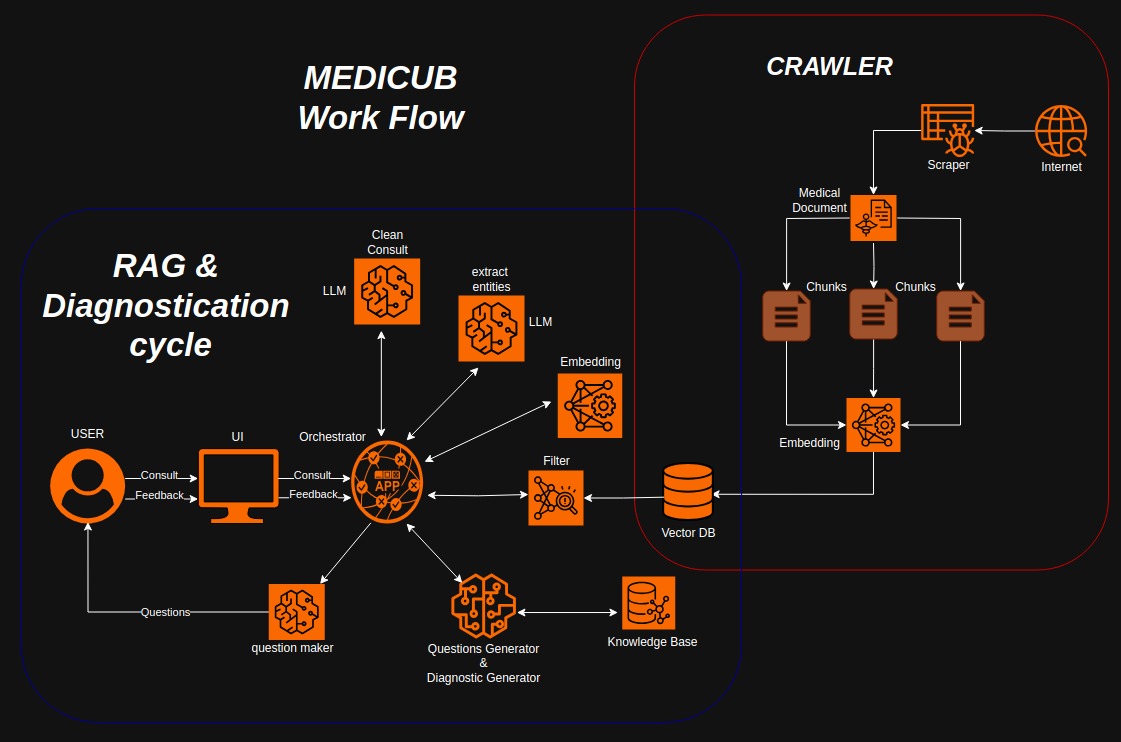
\includegraphics[scale=0.18]{Work Flow.png}
  \end{center}
  
  \begin{itemize}
    \item Orquestador
    \item Expansor de consulta
    \item Base de datos actualizada (Crawler)  
    \item Base de conocimiento (grafo médico)
  \end{itemize}

\end{frame}

\begin{frame}{Diagrama de componentes - Agentic RAG}
  \begin{center}
    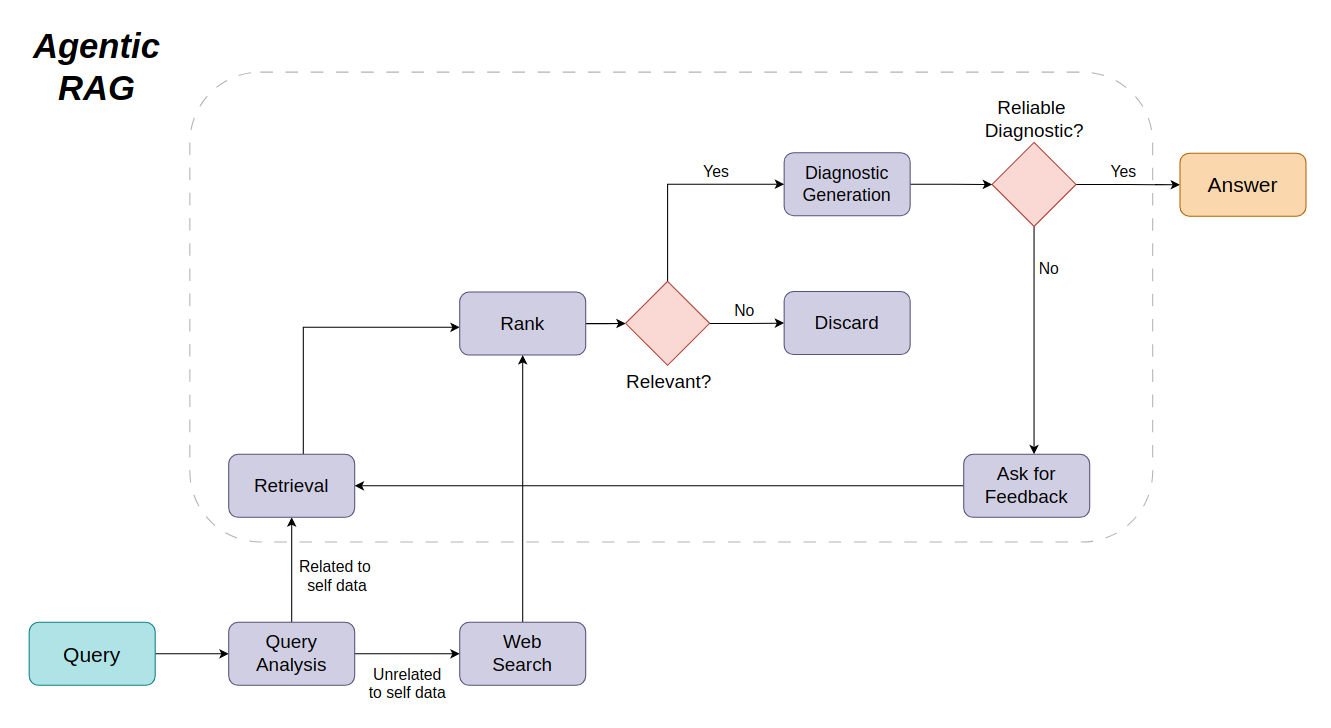
\includegraphics[scale=0.25]{Agentic_RAG.png}
  \end{center}  
\end{frame}

\begin{frame}{Diagrama de componentes - Diagnostic Architecture}
  \begin{center}
    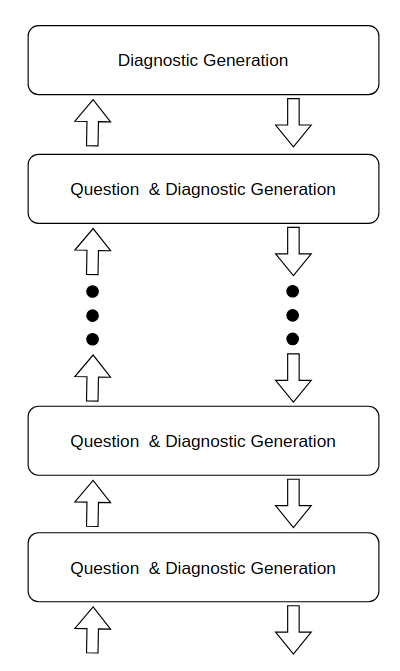
\includegraphics[scale=0.32]{Diagnostic_Layer_Architecture.png}
  \end{center}  
\end{frame}

\begin{frame}{Diagrama de componentes - Grafo de conocimiento}
  \begin{center}
    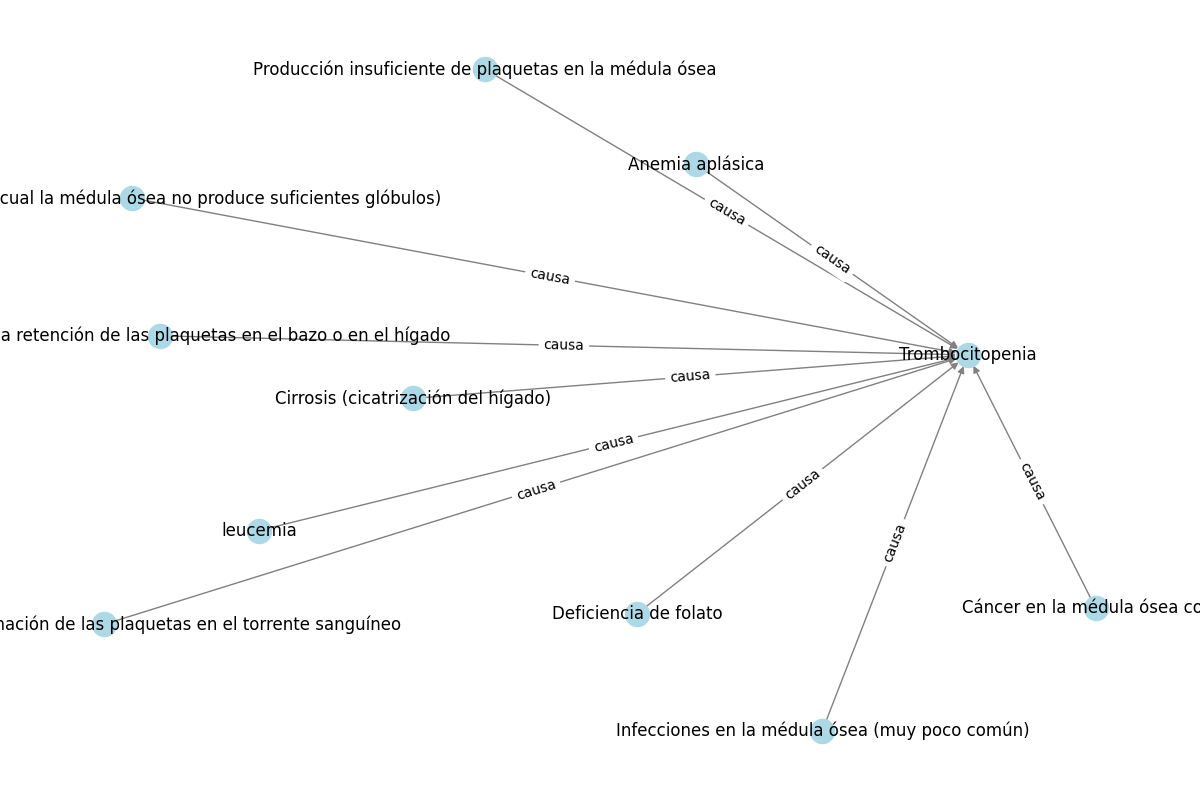
\includegraphics[scale=0.4]{graph_example.png}
  \end{center}  
\end{frame}


\begin{frame}{Futuras Mejoras}
    \begin{itemize}
        \item Integración con datos estructurados
        \item Expansión a otros idiomas
        \item Mejoras en el grafo de conocimiento médico
        \item Aumento en precisión de diagnóstico
    \end{itemize}
\end{frame}

\begin{frame}{Gracias}
    \centering
    \LARGE\textbf{Gracias!} \\
\end{frame}

\end{document}
